\chapter{Systemanalyse}\label{ch:systemanalyse}

\paragraph{Zielgrößen}
Die relevanten Zielgrößen werden mit der Methode Critical to Quality (CTQ) \cite{WiMa24} identifizieren.
Für CTQ gilt es die folgende Frage zu beantworten: 
Welche Eigenschaften machen einen Keks gut oder vergleichbar?
Die Eigenschaften werden gesammelt und kategorisiert.
Anschließend werden messbare Zielgrößen abgeleitet.
Die Kategorien und Zielgrößen sind auch in der Tabelle \ref{table:zielgroeßen}

\begin{table}[h!]
\centering
\caption{Kategorien und Zielgrößen aus der CTQ}
\label{table:zielgroeßen}
\begin{tabular}{|l|l|}
\hline
Kategorie  & Zielgrößen  \\
\hline
\textbf{Geometrie}  & \textbf{Durchmesser, Höhe, Ausbreitungsfaktor}\\
Masse  & Gewicht, Gewichtsverlust beim Backen \\
Struktur  & Härte, Knusprigkeit, Bruchkraft \\
Optik  & Bräunungsgrad, Rissbildung, Gleichmäßigkeit der Kontur \\
Sensorik  & Süße, Buttergeschmack, Mundgefühl \\
\hline
\end{tabular}
\end{table}

Eine erste Kategorie, die dabei auffällt, ist die Geometrie.
Durchmesser und Höhe des Cookies können einfach gemessen und verglichen werden.
Aus dem Durchmesser vor und nach dem Backen lässt sich der Ausbreitungsfaktor ableiten.
Ebenso einfach lässt sich das Gewicht des Cookie bestimmen.
Mit Messungen vor und nach dem Backvorgang kann so der Gewichtsverlust ermittelt werden.
Gewicht und Gewichtsverlust bilden dabei die Kategorie der Masse.
Eine dritte Kategorie ist die Struktur des Cookies.
Zielgrößen darin sind die Härte oder Knusprigkeit des Cookies sein.
Messbar werden die Zielgrößen mit der Bruchkraft.
Die Optik als vierte Kategorie umfasst den Bräunungsgrad, die Rissbildung und die Gleichmäßigkeit der Kontur.
Die letzte und wichtigste Kategorie ist die Sensorik.
Zu ihr gehören die Süße, der Buttergeschmack und das Mundgefühl.

Die Kategorie der Geometrie ist mit den limitierten Messmittel gut erfassbar.
Gleiches gilt für die Masse, die aufgrund von Komplexität aber ausgelassen wird.
FÜr die Struktur und Optik fehlen die nötigen Messmittel.
Die Sensorik kann über Menschen ausgewertet werden.
Sie unterliegen aber einem subjektiven Empfinden.
Die Werte sind dadurch weniger vergleichbar.

% SIPOC- oder Prozesskettenanalyse
% \begin{figure}
%     \centering
%     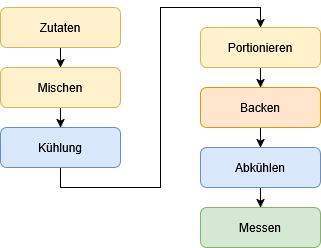
\includegraphics[width=\linewidth]{figures/prozess.png}
%     \caption{.}
%     \label{fig:prozess}
% \end{figure}
% Dann überlegst du pro Schritt, welche messbaren Merkmale entstehen oder beeinflusst werden.
% Beispiel:
% Prozessschritt	Mögliche Zielgröße
% Teig herstellen	Teigkonsistenz, Teigklebrigkeit, Teigtemperatur
% Portionieren	Rohteiggewicht, Rohteigdurchmesser
% Backen	Durchmesserzunahme, Höhenänderung, Bräunung
% Abkühlen	Endhöhe, Enddurchmesser, Festigkeit
% Lagerung	Feuchteverlust, Härtezunahme


\paragraph{Einfluss- und Störgrößen}

Zur Sammlung der Einfluss- und Störgrößen wird ein Ursache-Wirkungs-Diagramm \cite{Schu13} erstellt.
Bei der Erstellung des Diagramms werden alle Wirkungen auf ein Ziel identifiziert.
Die Wirkungen dienen zur Ableitung der Einfluss- und Störgrößen.
Das Ziel dieser Arbeit ist die Herstellung guter Cookies.
Die Hauptwirkungen auf das Ziel sind Material, Umwelt, Methoden, Maschine, Messung und Mensch.
Alle Nebenwirkungen sind in der Abbildung \ref{fig:ursache_wirkung} zu sehen.

\begin{figure}
    \centering
    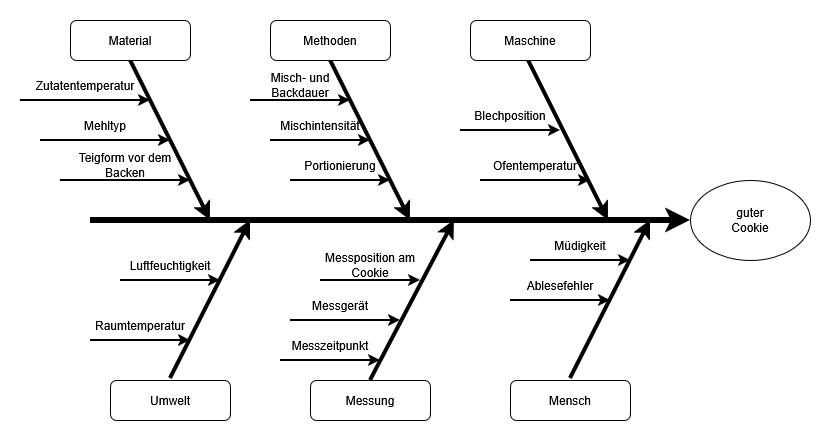
\includegraphics[width=\linewidth]{figures/ursachen-wirkungs-diagramm.drawio.png}
    \caption{Ursache-Wirkungs-Diagramm für gute Cookies.}
    \label{fig:ursache_wirkung}
\end{figure}

% \paragraph{P-Diagramm}

% Aus den gesammelten Größen lässt sich nun das Parameterdiagramm \cite{Sieb26} erstellen.
% Es teilt die Größen, die auf den Prozess wirken, in Signalgrößen, Steuergrößen, Störgrößen, Qualitätsmerkmale (hier Zielgrößen) und Error States.
% Die Abbildung \ref{fig:p_diagramm} zeigen die finale Einteilung der Größen.


\paragraph{Vorversuch}
Ein Vorversuch brachte wichtige Erkenntnisse. 
So wurden im Vorversuch Stückchen einer weißen Tafel Schokolade und Cranberries für die Cookies verwendet.
Die unterschiedlich großen Schokoladenstückchen und Cranberries führten zu starken variierenden Cookie-Formen.
Die Cookies aus dem Vorversuch sind in Abbildung \ref{fig:vorversuch} im Anhang \ref{ch:appendix_c} zu sehen.
Im Experiment werden deshalb Schokoladentropfen (SchokoTro) verwendet.
Diese sind maschinell gefertig und deutlich konsistenter in ihrer Größe.

Der Vorversuch nutzte zwei Extreme des Faktorraums.
Einen Teig mit 0\,\% Vollkornmehl, minimaler Zucker- und Buttermenge und ein Teig mit maximaler Zucker- und Buttermenge mit 0\,\% Vollkornmehl.
Dabei zeigten sich deutliche Unterschiede im Durchmesser und der Höhe der Cookies.
Es zeigte sich zudem, dass der Messzeitpunkt für den Durchmesser nach dem Backen nicht relevant ist.
Bei der Höhe sind 30 Minuten nach der Entnahme aus dem Ofen keine Änderungen messbar.